\chapter{The ML Workflow: End-to-End}
\label{chap:ml_workflow}

% ========================================
% SECTION 0: METADATA
% ========================================
% Prerequisites: None
% Learning Outcomes:
% - The 7 steps of a real-world ML project
% - Why 80% of time is Data Prep
% - Introduction to Sklearn Pipelines
% Interview Relevance: High (System Design)

% ========================================
% SECTION 1: MOTIVATION
% ========================================
\section{Motivation}
Junior engineers often think Machine Learning is just:
\begin{lstlisting}[language=Python]
model.fit(X, y)
model.predict(X_new)
\end{lstlisting}
In reality, this is only 5\% of the work. The other 95\% is understanding the problem, cleaning the mess (data), and keeping the system alive in production. If you skip the workflow, you build a garbage-in-garbage-out system.

% ========================================
% SECTION 2: INTUITION
% ========================================
\section{Intuition: The Master Chef}
Think of ML like a high-end restaurant kitchen:
\begin{enumerate}
    \item \textbf{Problem Def}: "We need a spicy vegan starter." (Customer Requirement)
    \item \textbf{Data Collection}: Sourcing ingredients (Vegetables, Spices).
    \item \textbf{Preprocessing}: Washing, chopping, peeling (Cleaning Data).
    \item \textbf{Training}: Cooking (The Algo).
    \item \textbf{Evaluation}: Tasting (Metrics).
    \item \textbf{Deployment}: Serving clearly on a plate (API).
\end{enumerate}
If you cook rotten vegetables (bad data) with a Michelin-star recipe (great model), the food significantly sucks.

% ========================================
% SECTION 3: VISUALIZATION
% ========================================
\section{The 7-Step Pipeline}
\begin{figure}[h]
    \centering
    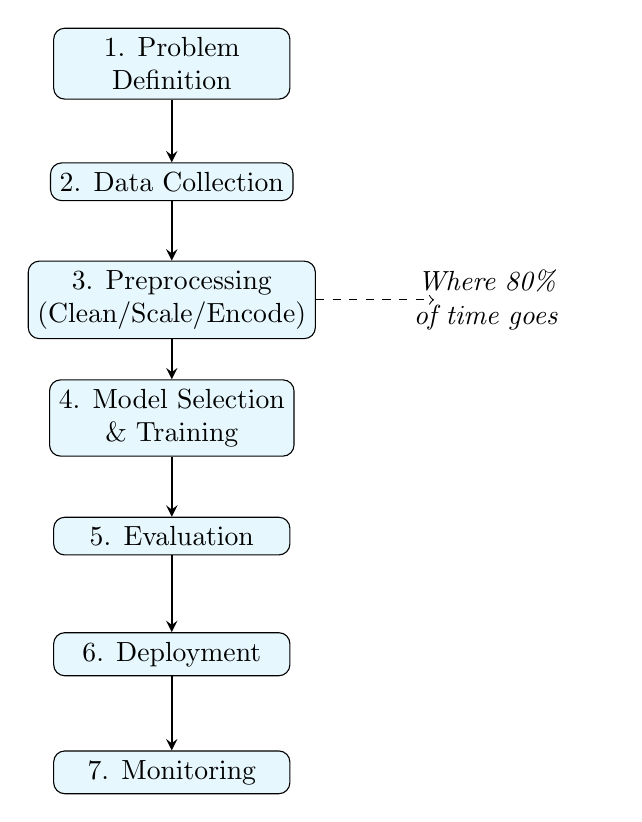
\begin{tikzpicture}[
        node distance=1.5cm,
        every node/.style={rectangle, rounded corners, draw=black, align=center, fill=cyan!10, minimum width=3cm},
        arrow/.style={thick, ->, >=stealth}
    ]
        \node (1) {1. Problem\\Definition};
        \node (2) [below of=1] {2. Data Collection};
        \node (3) [below of=2] {3. Preprocessing\\(Clean/Scale/Encode)};
        \node (4) [below of=3] {4. Model Selection\\\& Training};
        \node (5) [below of=4] {5. Evaluation};
        \node (6) [below of=5] {6. Deployment};
        \node (7) [below of=6] {7. Monitoring};
        
        \draw[arrow] (1) -- (2);
        \draw[arrow] (2) -- (3);
        \draw[arrow] (3) -- (4);
        \draw[arrow] (4) -- (5);
        \draw[arrow] (5) -- (6);
        \draw[arrow] (6) -- (7);
        
        \node [right of=3, xshift=2.5cm, draw=none, fill=none, text width=3cm] {\textit{Where 80\% of time goes}};
        \draw [dashed, ->] (3.east) -- +(1.5,0);
    \end{tikzpicture}
    \caption{The Real-World ML Lifecycle}
\end{figure}

% ========================================
% SECTION 4: THE STEPS DETAILED
% ========================================
\section{Step-by-Step Breakdown}

\subsection{1. Problem Definition}
Convert "Business Need" to "ML Task".
\begin{center}
\begin{tabular}{|l|l|}
\hline
\textbf{Business Goal} & \textbf{ML Problem} \\ \hline
Reduce Credit Risk & Binary Classification (Default Y/N) \\ \hline
Forecast Sales & Time-Series Regression \\ \hline
Group Customers & Clustering \\ \hline
\end{tabular}
\end{center}

\subsection{2. Preprocessing (The Grunt Work)}
\begin{itemize}
    \item \textbf{Missing Values}: Drop rows? Impute Mean? Impute Zero?
    \item \textbf{Encoding}: One-Hot (Nominal) vs Ordinal (Ordered).
    \item \textbf{Scaling}: Standard vs MinMax (See Chapter 0.3).
\end{itemize}

\subsection{3. Model Selection}
How to choose? Occam's Razor: Start Simple!
\begin{itemize}
    \item \textbf{Baseline}: Always start with Logistic Regression / Linear Regression.
    \item \textbf{Complexity}: Move to Random Forest / GBM only if baseline fails.
    \item \textbf{Deep Learning}: Only for Images/Text/Audio.
\end{itemize}

% ========================================
% SECTION 6: IMPLEMENTATION
% ========================================
\section{Python: Sklearn Pipelines}
The Pro Way: Use `Pipeline` to chain steps. Ensures no data leakage.

\begin{lstlisting}[language=Python, caption=The Modern Pipeline]
from sklearn.pipeline import Pipeline
from sklearn.impute import SimpleImputer
from sklearn.preprocessing import StandardScaler
from sklearn.linear_model import LogisticRegression

# Define the pipeline steps
pipe = Pipeline([
    ('imputer', SimpleImputer(strategy='mean')), # Step 1: Fill missing
    ('scaler', StandardScaler()),                # Step 2: Scale
    ('model', LogisticRegression())              # Step 3: Train
])

# Fit and Predict (Leakage-free!)
pipe.fit(X_train, y_train)
y_pred = pipe.predict(X_test)
\end{lstlisting}

% ========================================
% SECTION 7: PITFALLS
% ========================================
\section{Pitfalls}
\begin{itemize}
    \item \textbf{Premature Optimization}: Spending weeks tuning Hyperparameters on a model with bad data.
    \item \textbf{Metric Mismatch}: Optimizing Accuracy when the business cares about Recall (Fraud).
    \item \textbf{Deployment Gap}: Model works in Jupyter Notebook but fails in API (latency, version mismatch).
\end{itemize}

% ========================================
% SECTION 8: INTERVIEW QUESTIONS
% ========================================
\section{HOTS Questions}
\textbf{Q1: Walk me through your typical ML workflow.}
\begin{itemize}
    \item Start with Business Understanding $\rightarrow$ Data Collection $\rightarrow$ EDA $\rightarrow$ Preprocessing $\rightarrow$ Baseline Model $\rightarrow$ Complex Model $\rightarrow$ Evaluation $\rightarrow$ Deployment. Emphasize that you revisit steps (it's iterative).
\end{itemize}

\textbf{Q2: Why use a Pipeline instead of manual steps?}
\begin{itemize}
    \item Prevents Data Leakage (transforms test data using training stats).
    \item Makes code reproducible and cleaner.
    \item Allows Cross-Validation on the entire workflow (including preprocessing).
\end{itemize}

% ========================================
% SECTION 9: QUICK REFERENCE
% ========================================
\section{Quick Reference Card}

\begin{center}
\fbox{\parbox{0.9\textwidth}{
\textbf{ML WORKFLOW - CHEAT SHEET}
\vspace{0.3cm}

\textbf{The 3-Phase Rule}:
\begin{enumerate}
    \item \textbf{Data Phase} (80\%): Collect, Clean, Encode, Scale.
    \item \textbf{Model Phase} (15\%): Baseline First $\rightarrow$ Tune $\rightarrow$ Ensemble.
    \item \textbf{Ops Phase} (5\%): Deploy, Monitor, Retrain.
\end{enumerate}

\textbf{Sklearn Pipeline}:
\texttt{Pipeline([('name', Transform), ..., ('model', Estimator)])}

\textbf{Model Selection Guide}:
\begin{center}
\begin{tabular}{|l|l|}
\hline
\textbf{Data} & \textbf{Start With} \\ \hline
Tabular (Small) & Logistic/Linear Regression \\ \hline
Tabular (Medium) & Random Forest / XGBoost \\ \hline
Image/Text & Deep Learning (CNN/Transformer) \\ \hline
Unlabeled & K-Means / PCA \\ \hline
\end{tabular}
\end{center}

\textbf{Interview Gold}:
\begin{itemize}
    \item "I always establish a baseline first."
    \item "I spend most time on Data Quality."
    \item "Leakage is the enemy."
\end{itemize}
}}
\end{center}
